%%%%%%%%%%%%%%%%%%%%%%%%%%%%%%%%%%%%%%%%%%%%%%%%%%%%%%%%%%%%%%%%%%%%%%%%%%%%%
%	e-Yantra, IIT-Bombay

%	Document Author: Abhishek Rathore, Gopineedi Harsha Vardhan
%	Date: 07-June,2016 

%%%%%%%%%%%%%%%%%%%%%%%%%%%%%%%%%%%%%%%%%%%%%%%%%%%%%%%%%%%%%%%%%%%%%%%%%%%%%

\documentclass[11pt,a4paper]{article}

\usepackage{graphicx}
\usepackage{listings}
\usepackage{url}
\usepackage{hyperref}
\title{Tutorial - Colored object tracking using HSV}
\author{e-Yantra Team}
\date{\today}

\begin{document}
	\maketitle
	\newpage
	\tableofcontents
	\newpage
	\section{Objective}
	The objective of this tutorial is to track a colored object using a Camera/Webcam.
	\section{Prerequisites}
	User should have handy knowledge of the following for understanding this tutorial.
	\begin{itemize}
		\item Basics of Python.
		\item Basics of OpenCV.
		\item Basics of Image processing.
		\item Knowledge about BGR and HSV color spaces and conversions.
	\end{itemize}
	\section{Hardware Requirement}
	\begin{itemize}
		\item A Computer with an internal or external webcam.
	\end{itemize}
	\section{Software Requirement}
	\begin{itemize}
		\item Python 2.7.5
		\item OpenCV 2.4.9 
		\item numpy 1.7.1
		\item \textbf{Note :} These are the versions we were working on while creating this tutorial.
	\end{itemize}
	\section{Theory and Description}
	\begin{itemize}
		\item Object detection and segmentation is the most important and challenging fundamental task of computer vision.  It is a critical part in many applications such as image search, scene understanding, etc.The easiest way to detect and segment an object from an image is the color based methods . The object and the background should have a significant color difference in order to successfully  segment objects using color based methods.
		\item Here we are using HSV Colorspace for Object detection instead of RGB Colorspace because unlike RGB, HSV separates luma, or the image intensity, from chroma or the color information.By using HSV/HSL we can also remove intensity,lightness which is not possible in RGB colorspace.Moreover HSV can also detect skin color ,fire color etc. 
		\item  As every pixel in the frame has different HSV values,we threshold(mask) the object by extracting it using the HSV values of it.We do this by masking all pixels by setting value 1(white) that have the HSV value as of the object and other pixels in the frame to 0 .
		\item After getting the binary image,we find contours bounding the white blobs in the frame and find their respective areas.Among all the bounded contours,the contour with the largest area would be our colored object.
		\begin{figure}[h!]
		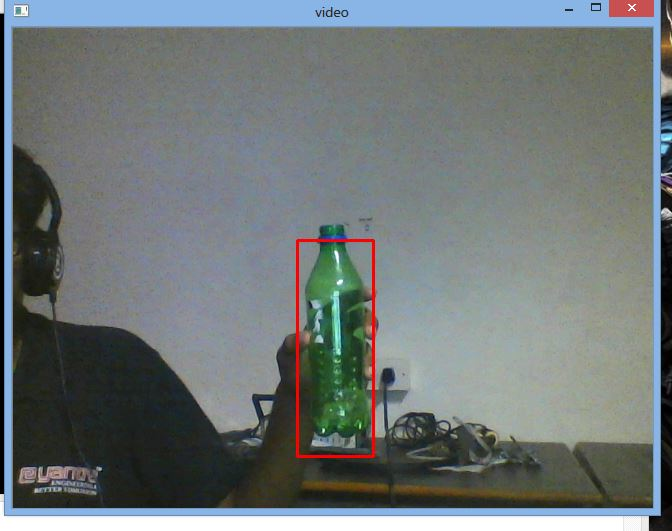
\includegraphics[scale=0.4]{Capture1.jpg}	
		\centering
		\caption{Masked image showing contours in the frame}
		\end{figure}
		\item Now we generate a boundary bounding that contour.In this way we can identify a colored object in a frame.By repeating this process in every frame we can track the object.Refer Figure 2		
		\begin{figure}[h]
		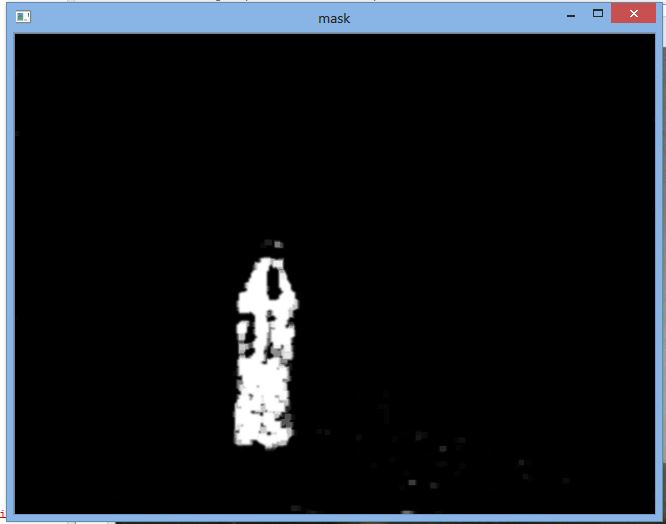
\includegraphics[scale=0.4]{Capture2.jpg}	
		\centering
		\caption{Boundary bounding the largest area contour}
		\end{figure}
		\item \textbf{Note :} This code works only, when your object (which you want to track) is the largest object of its color in the frame.Refer Figure 3.
		\begin{figure}[h!]
		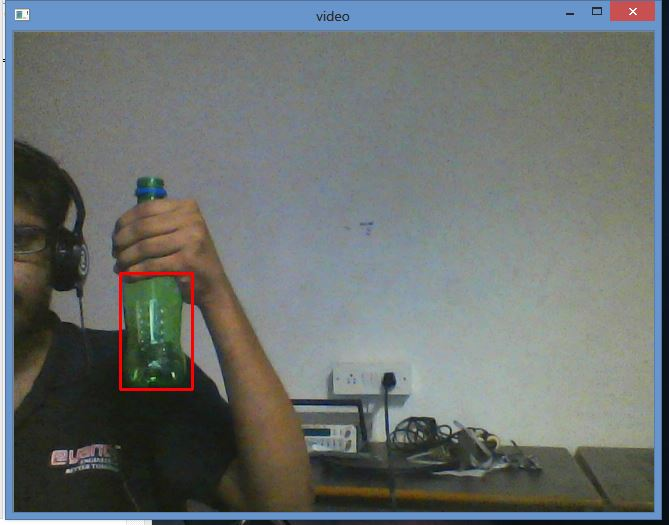
\includegraphics[scale=0.4]{Capture3.jpg}	
		\centering
		\caption{Boundary bounded on only one side of the bottle that has largest contour}
		\end{figure}
	\end{itemize}
	\newpage
	\section{Code}
    The Python code for this tutorial is available \href{https://github.com/eYSIP-2016/Object-Tracking-Camera/tree/master/Code/1.%20Colored%20Object%20Tracking%20using%20HSV}{here}
    \newpage
	\section{Exercise}
	Real time colored object tracking using webcam is shown below.
	\newline
	\newline
	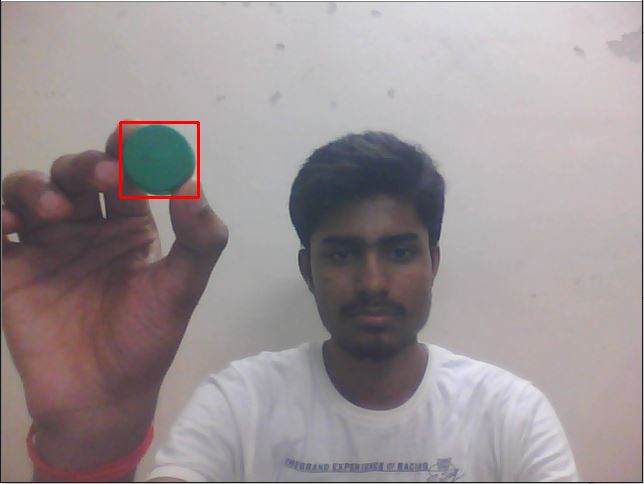
\includegraphics[scale=0.7]{image1.jpg}
	\newline
	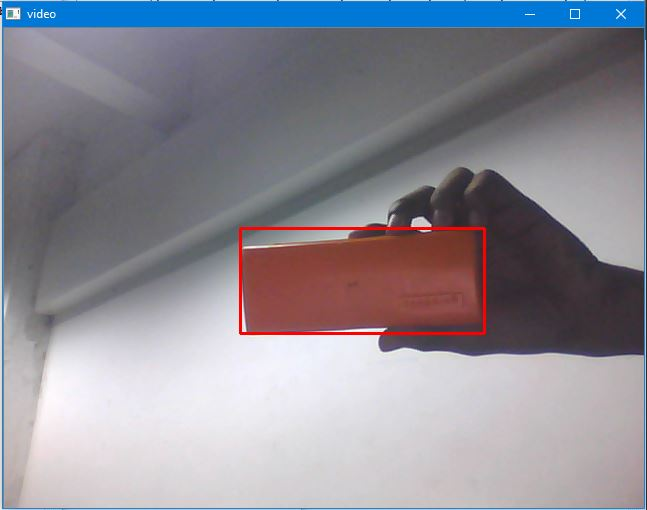
\includegraphics[scale=0.7]{image2.jpg}
	
	\section{References}
		\begin{enumerate}
			\item \url{https://opencv-python-tutroals.readthedocs.io/en/latest/py_tutorials/py_gui/py_drawing_functions/py_drawing_functions.html#drawing-functions}
			\item \url{https://opencv-python-tutroals.readthedocs.io/en/latest/py_tutorials/py_imgproc/py_colorspaces/py_colorspaces.html#converting-colorspaces}
			\item \url{https://opencv-python-tutroals.readthedocs.io/en/latest/py_tutorials/py_imgproc/py_filtering/py_filtering.html#filtering}
			\item \url{https://opencv-python-tutroals.readthedocs.io/en/latest/py_tutorials/py_imgproc/py_contours/py_contours_begin/py_contours_begin.html#contours-getting-started}
			\item \url{https://opencv-python-tutroals.readthedocs.io/en/latest/py_tutorials/py_imgproc/py_contours/py_contour_features/py_contour_features.html#contour-features}
		\end{enumerate}
			
\end{document}



